\chapter{Implementation}
\section{Development Process}

 \subsection{Initial Architecture Design}
The development process began with a modular architecture designed around four primary components, each with distinct responsibilities and well-defined interfaces:

\begin{itemize}
    \item Camera control system - Handles all camera interactions and image capture
    \item Dataset management - Manages data persistence and organization
    \item Analysis engine - Processes images and performs lens measurements
    \item User interface - Provides user interaction and result visualization
\end{itemize}

\subsection{Camera Integration Development}
The camera integration was implemented in three distinct phases:

\textbf{Phase 1: Basic Camera Communication}
\begin{itemize}
    \item Integration with gphoto2 library for camera control
    \item Implementation of basic camera connection/disconnection logic
    \item Development of camera status monitoring system
    \item Basic error handling and recovery mechanisms
\end{itemize}

\textbf{Phase 2: Advanced Camera Control}
\begin{itemize}
    \item Comprehensive camera settings management
    \item Manual and auto-focus control systems
    \item RAW format capture capabilities
    \item Real-time camera status monitoring
\end{itemize}

\textbf{Phase 3: Robustness Improvements}
\begin{itemize}
    \item Thread-safe camera operations
    \item Automatic camera reconnection handling
    \item Optimized memory management for image capture
    \item Timeout handling for camera operations
\end{itemize}

\subsection{Analysis Engine Development}
The analysis engine evolved through three main stages:

\textbf{Stage 1: Core Analysis Functions}
\begin{itemize}
    \item Raw image processing pipeline implementation
    \item MTF calculation algorithms
    \item Edge detection and analysis systems
    \item Basic lens distortion measurement %todo: prepisat
\end{itemize}

\textbf{Stage 2: Advanced Analysis Features}
\begin{itemize}
    \item Bokeh quality analysis implementation
    \item Chromatic aberration detection algorithms
    \item Vignetting measurement system
    \item Analysis result visualization generation
\end{itemize}

\textbf{Stage 3: Optimization}
\begin{itemize}
    \item Large image processing optimization
    \item Memory usage improvements
    \item Analysis accuracy refinements
    \item Multi-threaded analysis support
\end{itemize}

\subsection{Data Management Implementation}
The data management system was developed in two phases:

\textbf{Core Functionality}
\begin{itemize}
    \item Dataset creation and storage system
    \item Hierarchical file organization
    \item Comprehensive metadata management
    \item Analysis result storage
\end{itemize}

\textbf{Advanced Features}
\begin{itemize}
    \item Dataset import/export functionality
    \item Structured scenario management
    \item Analysis results comparison tools
    \item Data integrity verification systems
\end{itemize}

\subsection{Integration and Testing}
The integration process focused on two main areas:

\textbf{Component Integration}
\begin{itemize}
    \item Systematic core component integration
    \item Interface compatibility validation
    \item Performance optimization
    \item Resource management verification
\end{itemize}

\textbf{Testing Procedures}
\begin{itemize}
    \item Comprehensive unit testing
    \item Component integration testing
    \item Performance load testing
    \item UI functionality verification
\end{itemize}

\subsection{Deployment Considerations}
The final phase addressed deployment requirements:

\textbf{System Requirements}
\begin{itemize}
    \item Hardware compatibility testing
    \item Dependency management
    \item Installation process development
    \item System configuration management
\end{itemize}

\textbf{Documentation}
\begin{itemize}
    \item Technical documentation
    \item User guide creation
    \item API documentation
    \item Installation guides
\end{itemize}

\section{Used Technologies} %todo rozpisat

\subsection{Dependencies}
This project relies on Python programming language and on several Python libraries and tools:

\begin{itemize}
    \item \textbf{gphoto2}: Core library for camera communication and control
    \item \textbf{OpenCV}: Image processing and analysis capabilities
    \item \textbf{NumPy}: Numerical computations and array operations
    \item \textbf{rawpy}: RAW image file processing
    \item \textbf{NiceGUI}: Web-based user interface framework
\end{itemize}

\subsection{Development Environment}
The development environment integrates tools and configurations to support efficient and organized software development. Git is utilized for version control, enabling tracking of code changes. The primary platform for development is Linux, providing a robust and versatile foundation. Python virtual environments are employed to isolate dependencies. Additionally, an automated testing framework is incorporated to streamline testing, validate functionality, and maintain code quality.

\section{Implementation of System Components}

\subsection{Camera Control System}
The implementation of the camera control system is encapsulated within the CameraManager class, developed using the gphoto2 Python library. The CameraManager begins by initializing the camera context and establishing a connection using thread-safe locks. It ensures robust operation by continuously monitoring the camera's connection status and managing reinitialization when required.

Key features of the CameraManager include the ability to list all available camera properties through a recursive exploration of the camera's configuration widgets. It allows dynamic adjustments to parameters like aperture, ISO, shutter speed, and exposure modes.

The class also provides a mechanism for extracting metadata from images, leveraging EXIF data to gather information such as focal length, lens type, and exposure settings.

The image capture functionality includes autofocus handling and respect for existing camera settings. The captured images, along with their associated metadata, are stored systematically, facilitating subsequent analysis.

Error handling is a critical aspect of the camera control system. It manages hardware exceptions and unexpected states, such as camera unavailability, by logging detailed error messages and retrying operations where appropriate.

\subsection{Image Processing Pipeline}
The image processing pipeline processes calibration images to extract relevant optical properties of camera lenses, including sharpness, vignetting, distortion, chromatic aberrations, and bokeh.

\subsubsection{Image Preprocessing and Segmentation}

The implementation begins with an initial segmentation phase, which identifies calibration elements within the image. Using algorithms such as SIFT, the pipeline detects and localizes key graphical features of the test charts. This step establishes a foundation for subsequent stages by eliminating irrelevant areas of the image.

The next step is preprocessing, where a series of transformations is applied to normalize the data. Preprocessing tasks include noise reduction, image resizing, and contrast adjustment to account for variations in lighting and camera settings. The use of median or Gaussian filters ensures that these transformations preserve critical details. The pipeline also converts raw image data to an analyzable format.

\subsubsection{Feature Detection and Analysis}

The next stage evaluates specific lens properties. For sharpness, edge detection techniques are applied, enabling the analysis of transitions between high-contrast regions. The modulation transfer function (MTF) is calculated to quantify spatial resolution, providing a robust measure of lens clarity. Vignetting is assessed by analyzing the intensity distribution across the image, while geometric distortion is evaluated by comparing expected grid patterns to their actual appearance. Chromatic aberrations are quantified by measuring color fringing at the boundaries of high-contrast features, and bokeh quality is examined through the characterization of out-of-focus light regions.

A key characteristic of the pipeline is its adaptability to various calibration test charts and environmental conditions. This is achieved through parameterized algorithms and automated calibration routines. The pipeline also integrates mechanisms to validate the reliability of the extracted data, detecting and discarding outliers that might result from erroneous inputs.

The processed data is formatted for visualization and reporting. Analytical results are structured into metrics and graphs. The results are also stored for future reference.

\subsection{User Interface Components}
The application’s user interface provides tools for camera control, dataset management, and lens analysis. Users can connect cameras, adjust settings, capture images, and manage batch processes with real-time progress updates. Analysis tools display metrics and visualizations for sharpness, vignetting, distortion, chromatic aberrations, and bokeh. The UI also includes logging, notifications, and metadata visualization.

\subsubsection{Camera Control Panel}
The camera control panel offers a centralized interface for managing camera operations. Users can connect and disconnect the camera and monitor its status in real-time. Advanced camera controls include access to settings like aperture, shutter speed, and ISO. The application supports both automatic and manual focus adjustments, ensuring flexibility for various testing scenarios. Additional features include capturing images directly through the interface, importing RAW files, and listing all camera properties.

\begin{figure}[h]
\centering
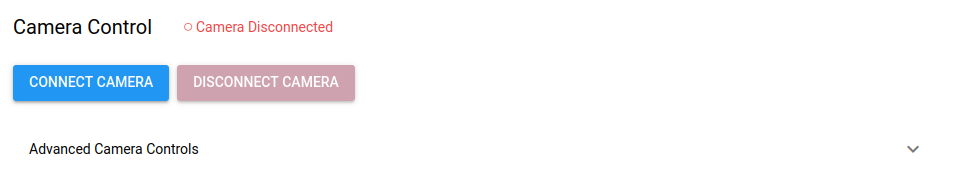
\includegraphics[width=1\textwidth]{Images/camera_control.png}
\caption{Camera control panel.}
\label{fig:ui_camera_control}
\end{figure}

\subsubsection{Datasets Panel}
The dataset panel enables handling captured images and related metadata. Users can import, create, select, and manage datasets, enabling systematic storage and categorization of images. Each image is linked to a specific scenario, allowing users to structure their tests based on various lens properties. Metadata embedding ensures that all relevant information, including camera settings and capture details, is preserved for future reference. The system also supports structured file naming conventions and temporary storage management, ensuring consistency and ease of navigation.

\begin{figure}[h]
\centering
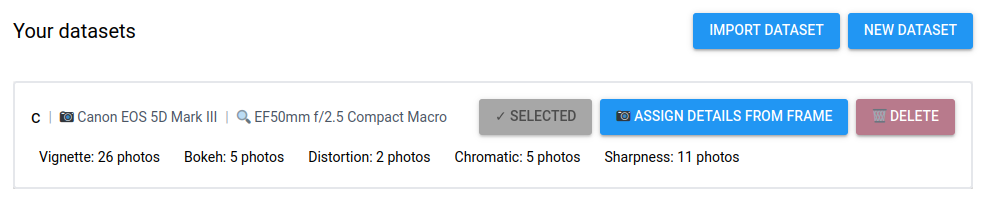
\includegraphics[width=1\textwidth]{Images/datasets_panel.png}
\caption{Datasets panel.}
\label{fig:ui_datasets}
\end{figure}

\subsubsection{Scenarios Panel} % todo
The scenarios panel allows users to target lens evaluations to specific properties, such as sharpness, vignetting, distortion, chromatic aberrations, and bokeh. Each scenario is linked to a dataset and includes predefined settings and workflows for capturing and analyzing images.

\begin{figure}[hbt]
\centering
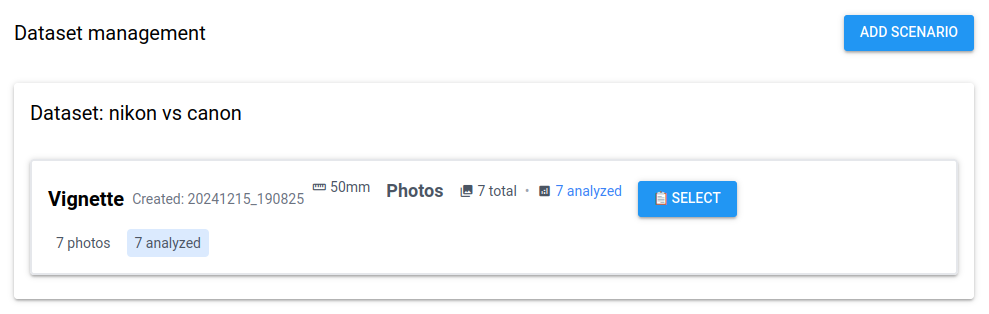
\includegraphics[width=1\textwidth]{Images/scenarios_panel.png}
\caption{Scenarios panel.}
\label{fig:ui_scenarios}
\end{figure}

The user can view detailed analysis results presented in a structured format. At the top, the Capture Settings section summarizes the camera configuration during the image capture. This includes details such as the camera model, lens information, aperture setting, shutter speed, ISO sensitivity, and focal length. These settings provide context for understanding the conditions under which the analysis was performed.

\begin{figure}[hbt]
\centering
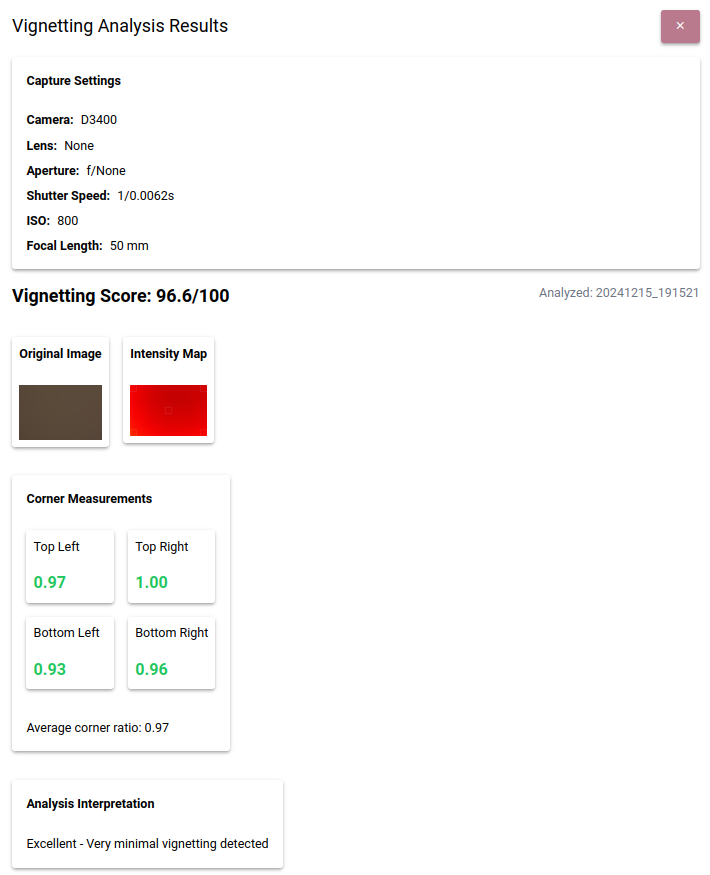
\includegraphics[height=0.8\textwidth]{Images/scenario_result.png}
\caption{Result of vignette scenario.}
\label{fig:ui_scenario_result}
\end{figure}

The Numerical Scores section delivers a quantitative assessment tailored to the specific scenario. For example, in sharpness analysis, this may include metrics like Modulation Transfer Function (MTF) scores. These scores are often normalized to a scale (e.g., 0-100) to simplify interpretation and enable comparisons across different lenses and settings.

The Visual Outputs section includes graphical representations to enhance the understanding of the analysis results. This may involve the display of the original captured image alongside processed visualizations, such as heatmaps, intensity maps and edge overlays.

The Measurement Details section provides more granular insights. This could include corner measurements for luminance ratios in vignetting analysis or edge intensity values for sharpness.

Finally, the Analysis Interpretation section summarizes the findings in plain language, offering a qualitative assessment of the results. For example, it may indicate whether vignetting is minimal, sharpness is excellent, or distortions are significant. This summary helps users quickly grasp the outcome of the analysis without needing to interpret the raw data or metrics.



\textbf{Vignetting} analysis results include center-to-corner luminance ratios, average corner intensity and a normalized vignetting score. Heatmaps visually represent brightness variations across the image and offer further insights into the vignetting effect.

\begin{figure}[hbt]
\centering

\includegraphics[width=0.4\textwidth]{Images/vignette_image_result.png}
\caption{Intensity map for vignette scenario.}
\label{fig:ui_vignette_intensity_map}
\end{figure}

For \textbf{sharpness} analysis, the UI displays numerical metrics such as Modulation Transfer Function (MTF) scores, edge intensity, and an overall sharpness rating. These are accompanied by graphs illustrating MTF curves across spatial frequencies and edge detection overlays that highlight areas of detail within the image. Original and processed images are shown side by side, providing clear visual comparisons.

\begin{figure}[h]
\centering
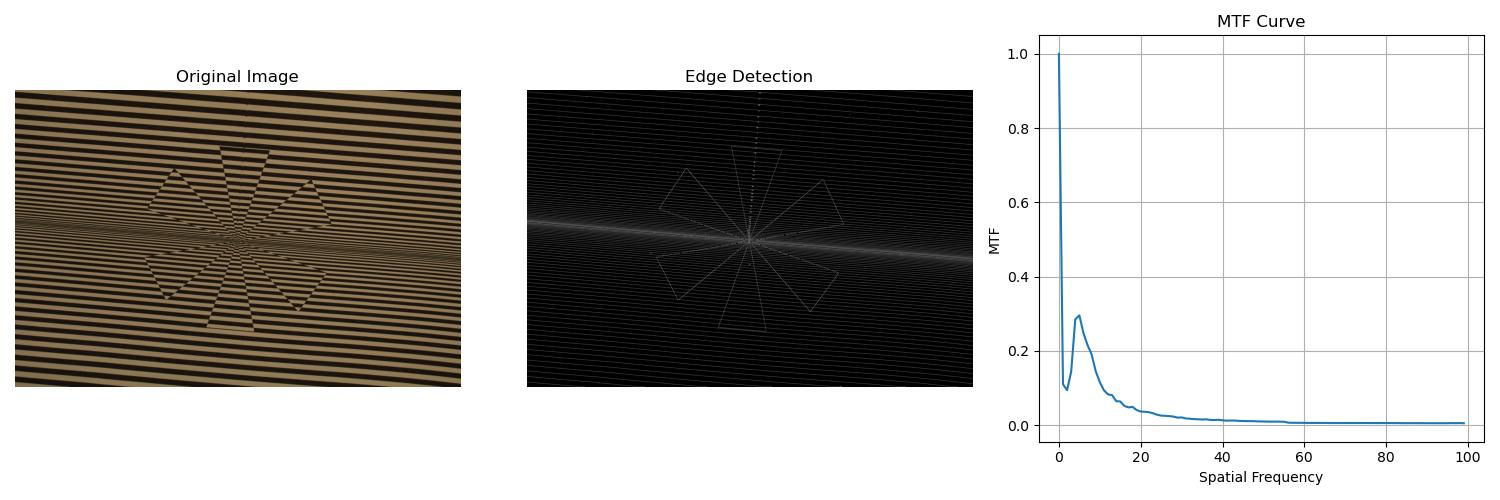
\includegraphics[width=1\textwidth]{Images/sharpness_image_result.jpg}
\caption{Sharpness analysis details.}
\label{fig:ui_sharpness_image}
\end{figure}

For \textbf{distortion} analysis, the system outputs metrics such as deviations in line straightness, average line deviation, and an overall distortion score. Grid overlays on the original image demonstrate detected distortion patterns, while corrected and uncorrected versions are displayed for comparison. The type of distortion—barrel, pincushion, or waveform—is identified based on the analysis.

\textbf{Chromatic aberration} analysis highlights color fringing in images, providing metrics on pixel offsets and scores for lateral and longitudinal aberrations. The UI displays zoomed-in sections of the image where chromatic aberrations occur, with overlaid color error vectors for visualization. Original and corrected images are presented side by side to showcase the impact of corrections.

In \textbf{bokeh} analysis, the system evaluates characteristics such as roundness, smoothness, and consistency of out-of-focus highlights. Overlays highlight bokeh regions, accompanied by metrics for size, shape, and edge definition. Users can compare bokeh characteristics across different aperture settings or light sources using dynamic visualization tools.

\begin{figure}[h]
\centering
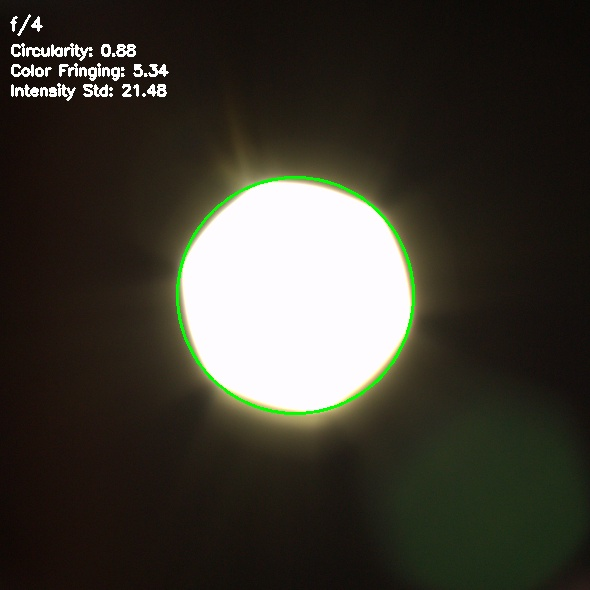
\includegraphics[width=0.3\textwidth]{Images/bokeh_image_result.jpg}
\caption{Bokeh analysis details.}
\label{fig:ui_bokeh_image}
\end{figure}

\subsubsection{System Logs}
The system logs provide a real-time record of application activities, ensuring transparency and aiding in troubleshooting. Logs capture key events such as camera connections, configuration changes, capture processes, and errors. Displayed within the user interface, the logs update dynamically, allowing users to monitor the status of ongoing tasks.

\begin{figure}[h]
\centering
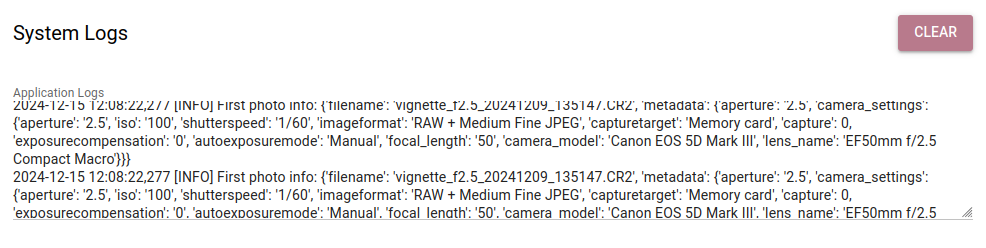
\includegraphics[width=1\textwidth]{Images/system_logs.png}
\caption{System logs.}
\label{fig:ui_system_logs}
\end{figure}

\subsubsection{Notifications}
The notification system provides real-time feedback to users. Notifications appear dynamically within the user interface to report critical events, such as successful camera connections and image captures. They also alert users to errors, including connection failures, invalid configurations, or file transfer issues.

\begin{figure}[h]
\centering

\includegraphics[width=0.7\textwidth]{Images/notification.png}
\caption{Notification example.}
\label{fig:ui_notification}
\end{figure}

%% BIG IMAGES
\begin{figure}[hbt]
\centering
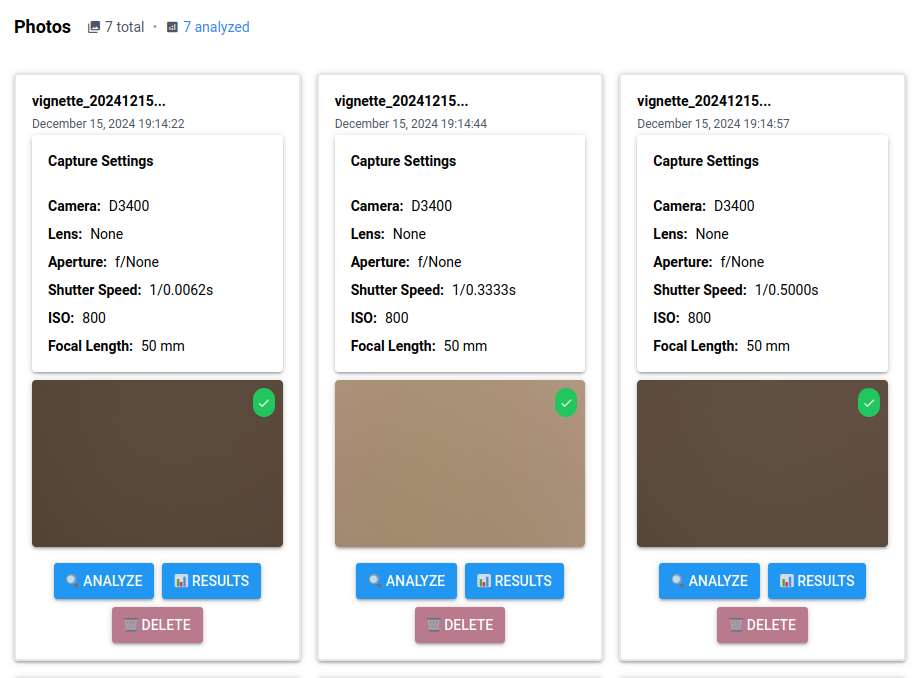
\includegraphics[width=0.8\textwidth]{Images/scenario_photos.png}
\caption{Overview of scenario's images.}
\label{fig:ui_scenario_images}
\end{figure}

\subsection{Additional Features}
The application includes several key features that enhance user experience and functionality:
\begin{itemize}
    \item \textbf{Offline Operation}: The application can operate fully offline after the initial installation, allowing users to utilize its features without internet connectivity.
    \item \textbf{Dark Mode}: The application includes a dark mode feature, enhancing usability in low-light environments and providing a more comfortable viewing experience.
    \item \textbf{UI State Storage}: The application stores user interface state, including user preferences and the currently opened elements, between visits, ensuring a seamless user experience.
\end{itemize}

\section{Testing}

To ensure the reliability and correctness of the application, particularly in the context of the "garage lab" approach described in the methodology, a comprehensive test suite was implemented using the pytest framework. The tests were designed to validate both the technical functionality and the practical usability of the application.

\subsection{Test Architecture}
The test suite is organized into four main components, reflecting the modular architecture of the application:
\begin{itemize}
    \item \texttt{test\_camera\_manager.py} - Validates camera control and image acquisition
    \item \texttt{test\_dataset\_manager.py} - Ensures proper data organization and persistence
    \item \texttt{test\_analysis.py} - Verifies image processing and lens measurement algorithms
    \item \texttt{test\_ui.py} - Tests user interface components and interactions
\end{itemize}

\subsection{Camera Manager Tests}
The camera manager tests focus on ensuring reliable camera operation in various scenarios. They evaluate the initialization process and connection management, verify the accuracy and consistency of image capture and metadata extraction, and test the configuration of the camera for different testing scenarios. Additionally, these tests validate the processing of EXIF data to extract detailed lens information and assess the effectiveness of error handling and recovery mechanisms.

\subsection{Dataset Manager Tests}

The dataset tests evaluate the core functionalities of the DatasetManager class, ensuring proper management of datasets and their associated scenarios. They verify the creation, listing, updating, and deletion of datasets, as well as the addition and modification of scenarios within datasets. Additionally, they test the export and import capabilities to confirm that datasets are correctly archived and restored with all metadata and content.

\subsection{Analysis Tests}
The analysis tests validate various functionalities of the lens measurement algorithms, ensuring accurate evaluation of lens properties. The tests cover sharpness analysis, distortion measurement, vignetting detection, chromatic aberration evaluation, and bokeh analysis. They validate methods for detecting edges, calculating modulation transfer functions (MTF), analyzing visual artifacts, and generating visualizations. Additionally, preprocessing of RAW images, feature extraction, and score calculation for lens performance are tested..

\subsection{UI Tests}
The UI tests focus on ensuring the functionality, responsiveness, and reliability of the user interface in managing camera operations, datasets, and scenarios. These tests validate the integration of UI components with backend functionality, covering critical workflows such as camera connection, configuration, photo capture, and metadata visualization. They evaluate the behavior of UI elements like buttons, dialogs, and status indicators under different conditions, including error states. Additionally, the tests verify that key user actions (such as dataset and scenario creation, RAW file import, and analysis result display) operate seamlessly. Mocked components are used to simulate interactions, ensuring the interface handles real-world scenarios and unexpected events effectively.

\subsection{Test Fixtures and Mocking}
To facilitate reliable software testing within the "garage lab" approach, the test suite employs a range of fixtures and mocking techniques. Key test fixtures include:

\begin{itemize}
    \item \texttt{mock\_camera} - Simulates camera behavior
    \item \texttt{mock\_camera\_manager} - Provides camera control testing
    \item \texttt{temp\_dir} - Manages test file storage
    \item \texttt{dataset\_manager} - Handles test data organization
    \item \texttt{sample\_image} - Provides standardized test images
\end{itemize}

External dependencies, such as camera operations and file system interactions, are mocked to ensure consistency and reproducibility. Similarly, UI components are simulated to validate user interactions, while image processing operations rely on controlled test data to maintain accuracy and isolate external influences. These strategies enable thorough and reliable testing in a constrained, repeatable environment.

\subsection{Quality Assurance}
The test suite ensures quality assurance across multiple dimensions to verify the robustness and reliability of the application. 

\textbf{Functional testing} focuses on evaluating the core features, such as camera control reliability, accurate data management, precise analysis algorithms, and a responsive, user-friendly interface. 

\textbf{Error handling} is assessed by simulating common issues like camera connection failures, invalid user inputs, resource constraints, and potential data corruption  to ensure graceful recovery and stability. 

\textbf{Performance testing} evaluates the efficiency of image processing algorithms and optimization of memory usage, measures application response times, and confirms that resources are effectively cleaned up after operations. 

Together, these tests provide a comprehensive framework to validate the functionality, reliability, and performance of the application under diverse conditions. Test coverage reports are generated using pytest-cov to ensure comprehensive testing of all components, with particular attention to critical paths in the lens measurement workflows.


